\documentclass{beamer}

\mode<presentation>
{
	\usepackage{StyleFiles/Rome}
	\setbeamercovered{transparent}
}

\mode<handout>
{
	\usepackage{pgfpages}
	\pgfpagesuselayout{2 on 1}[a4paper,border shrink=5mm]
	\nofiles
}

\usepackage[english]{babel}
\usepackage[latin1]{inputenc}
\usepackage{dsfont}
\usepackage{setspace}
\usepackage{marvosym}
\usepackage[algoruled]{algorithm2e}
\usepackage{algorithmic,algorithm2e,float}

\setbeamertemplate{itemize subitem}{\tiny\raise1.5pt\hbox{\donotcoloroutermaths$ \blacktriangleright $}}

\definecolor{darkgreen}{RGB}{0,180,0}
\definecolor{lightred}{RGB}{210,0,0}

\title[Disambiguating Localization Symmetry Through a M-C PF]{\Large Disambiguating Localization Symmetry Through a Multi-Clustered Particle Filtering}

\subtitle{}

\author[Fabio Previtali]{\small\textbf{Fabio Previtali}\\Guglielmo Gemignani\\Luca Iocchi\\Daniele Nardi}

\date[September 16, 2015]{\scriptsize International Conference on Multisensor Fusion and Integration for Intelligent Systems\\San Diego, USA}

\begin{document}

\begin{frame}[plain]
	\titlepage
\end{frame}

\section{Introduction}

\begin{frame}
	\frametitle{Challenging Problem}
	
	\begin{center}
		\begin{tikzpicture}
			\node at (0,0) [draw=white,ultra thick,inner sep=0pt]
			{
				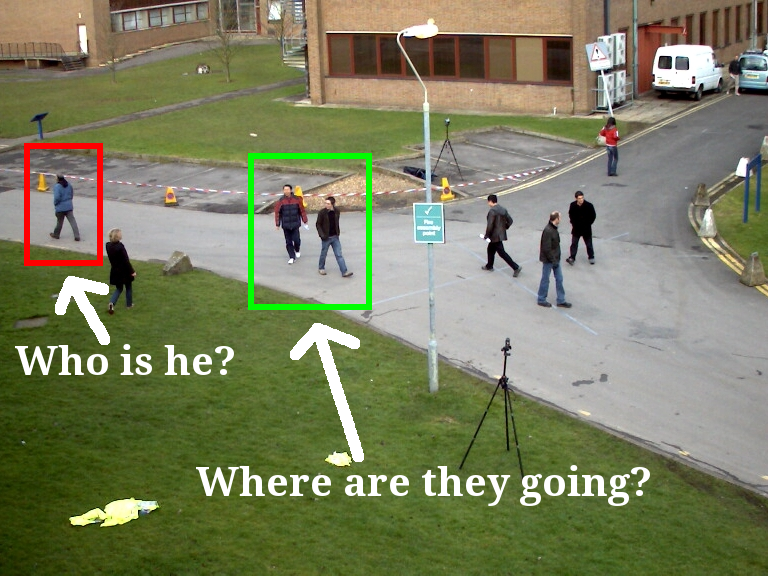
\includegraphics[width=\linewidth]{Figures/Problem.png}
			};
		\end{tikzpicture}
	\end{center}
\end{frame}

\begin{frame}
	\frametitle{Motivation}
	
	\vspace{0.2cm}
	
	\Large
	
	\begin{block}{Objective}
		\textbf{Understanding} the concept of human preference \textbf{allows} to perform higher levels
		of reasoning about future human actions. Likewise, the \textbf{knowledge} of a goal also gives
		information about \textbf{what} a person might do
	\end{block}
	
	\vspace{0.3cm}
	
	Example of application fields:
	\begin{itemize}
		\item Automatic video surveillance
		\item Human-Robot Interaction
		\item Domestic robots
	\end{itemize}
\end{frame}

\begin{frame}
	\frametitle{Contributions}
	
	\Large
	
	The main contributions of this thesis are:
	
	\begin{enumerate}
		\item \textbf{Distributed real-time} multiple object tracking
		\item \textbf{Asynchronous} and \textbf{fully} scalable design
		\item \textbf{Prediction} without prior scene semantics knowledge
		\item \textbf{Incremental} updates of the \emph{IRL} model over time
		\item \textbf{Non-uniform grids} for representing world state
		\item \textbf{Efficient} and \textbf{scalable} solution for on-robot implementation
	\end{enumerate}
\end{frame}

\begin{frame}
	\frametitle{Proposed Solution}
	
	\vspace{0.5cm}
	
	\begin{tikzpicture}
		\node at (0,0) [draw=white,ultra thick,inner sep=0pt]
		{
			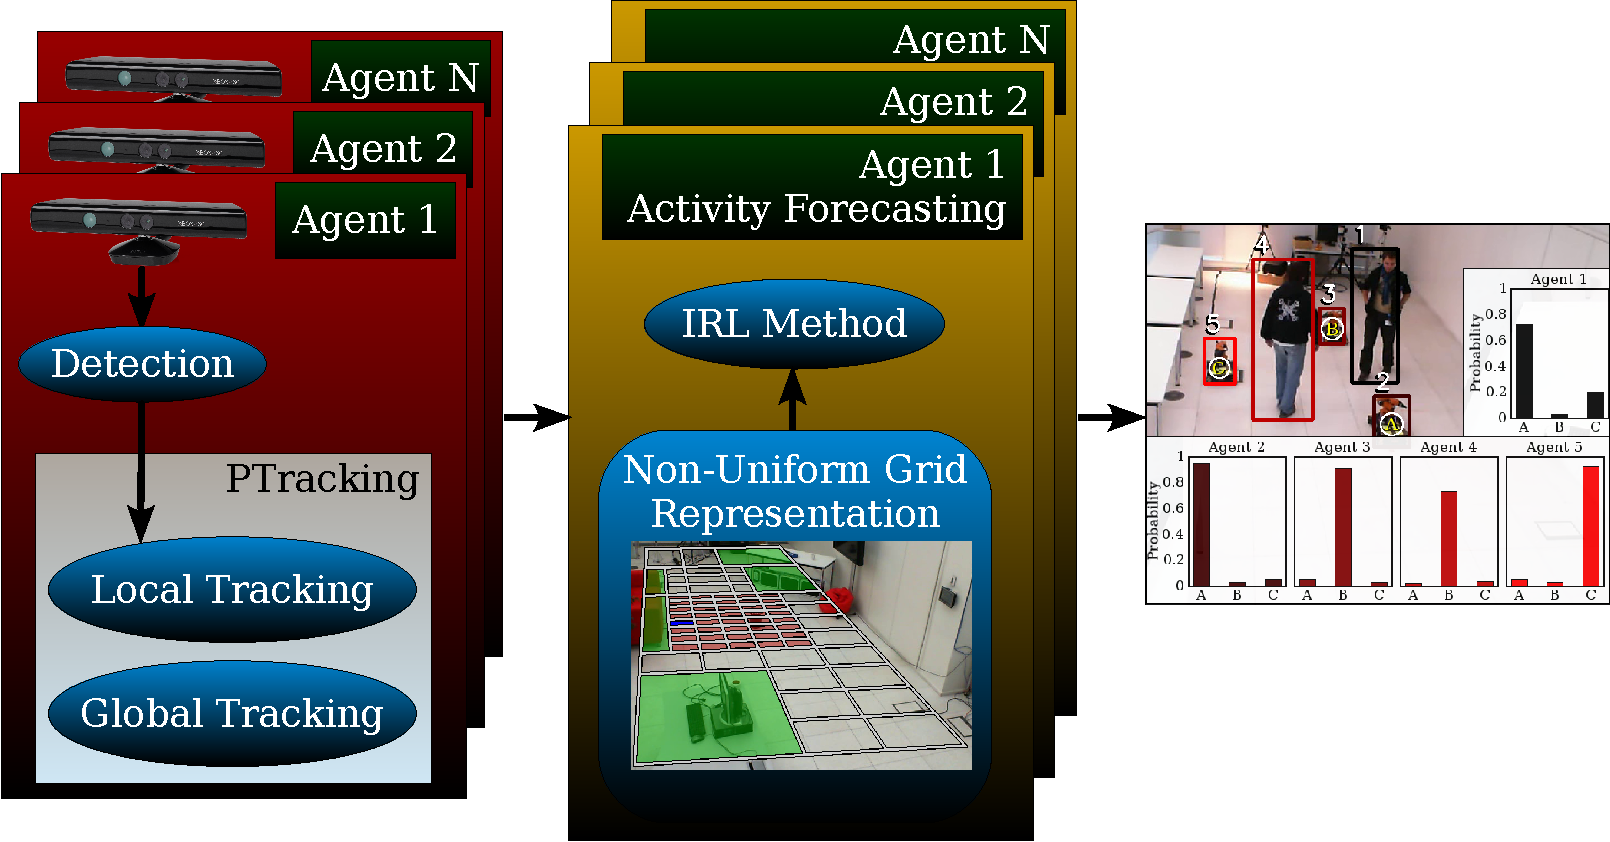
\includegraphics[width=\linewidth]{Figures/Architecture}
		};
	\end{tikzpicture}
\end{frame}

\section{PTracking Algorithm}

\begin{frame}
	\frametitle{}
	
	\Huge
	
	\vspace{0.5cm}
	
	\begin{center}
		\textbf{PTracking}
	\end{center}
\end{frame}

\begin{frame}
	\frametitle{PTracking}
	\framesubtitle{Distributed Particle Filtering for Multi-Sensor Multiple Object Tracking}
	
	\LARGE
	
	\begin{block}{Idea}
		Achieving \textbf{high} precision and robustness, as a global method does, while trying to keep
		a \textbf{low} computational load in order to obtain \textbf{real-time} performance, as
		recursive methods do
	\end{block}
\end{frame}

\begin{frame}
	\frametitle{PTracking}
	\framesubtitle{Contributions}
	
	\Large
	
	\vspace{0.2cm}
	
	We propose a novel technique based on \emph{Distributed Particle Filtering}. The key contributions
	are:
	
	\vspace{0.15cm}
	
	\begin{enumerate}
		\item \textbf{Real-time} multiple object tracking method
		\item Novel clustering method that \textbf{keeps} track of multiple objects whose number is
			  \textbf{not known} a priori, ensuring a \textbf{limited} Gaussian distribution in the
			  particle space
		\item \textbf{Asynchronous} algorithm to improve robustness with respect to communication
			  failures and dead nodes
	\end{enumerate}
\end{frame}

\begin{frame}
	\frametitle{PTracking}
	\framesubtitle{General Schema}
	
	\vspace{-0.27cm}
	
	\begin{columns}[T]
		\column{.5\textwidth}
		
		\vspace{0.8cm}
		
		\begin{itemize}
			\item \textbf{Input:} set of positions of the objects provided by a multi object detector
				  system (e.g., \cite{Bloisi12})
			
			\vspace{1.6cm}
			
			\item \textbf{Output:} set of estimated trajectories of the moving objects over time
		\end{itemize}
		
		\column{.5\textwidth}
		\centering
		
		\begin{tikzpicture}
			\node at (0,0) [draw=black,ultra thick,inner sep=0pt]
			{
				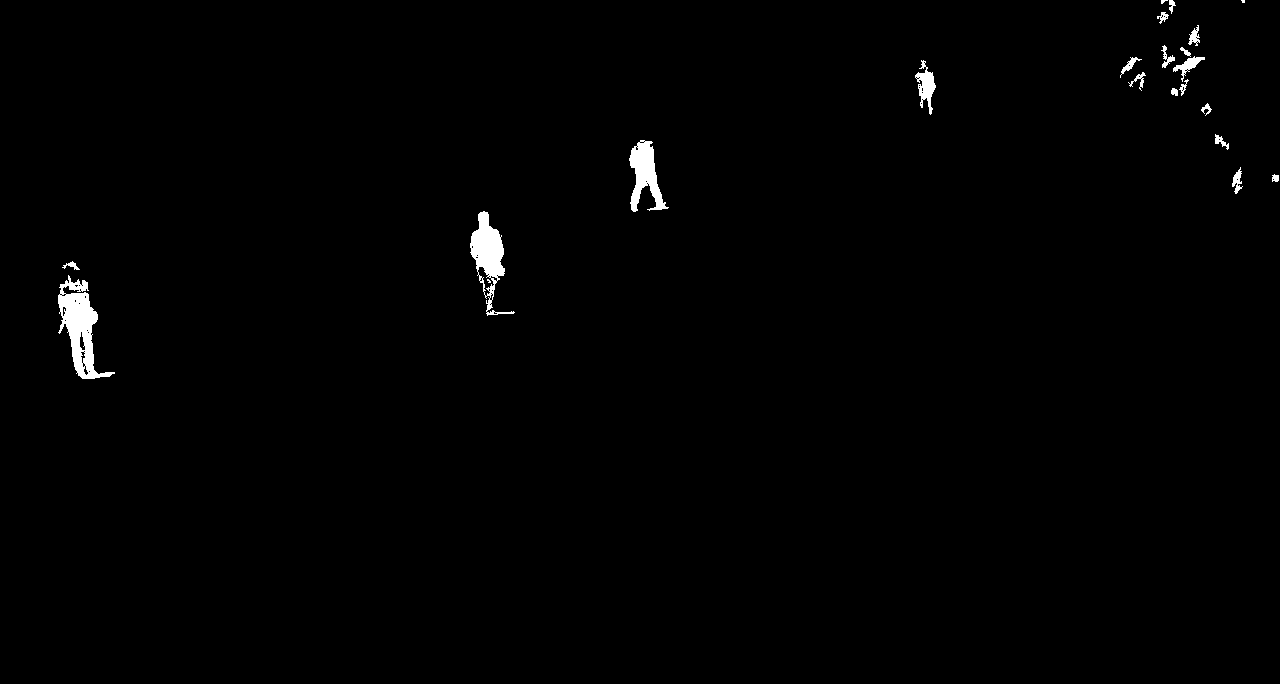
\includegraphics[width=6cm]{Figures/Detection}
			};
			\node at (0,-3.35) [draw=black,ultra thick,inner sep=0pt]
			{
				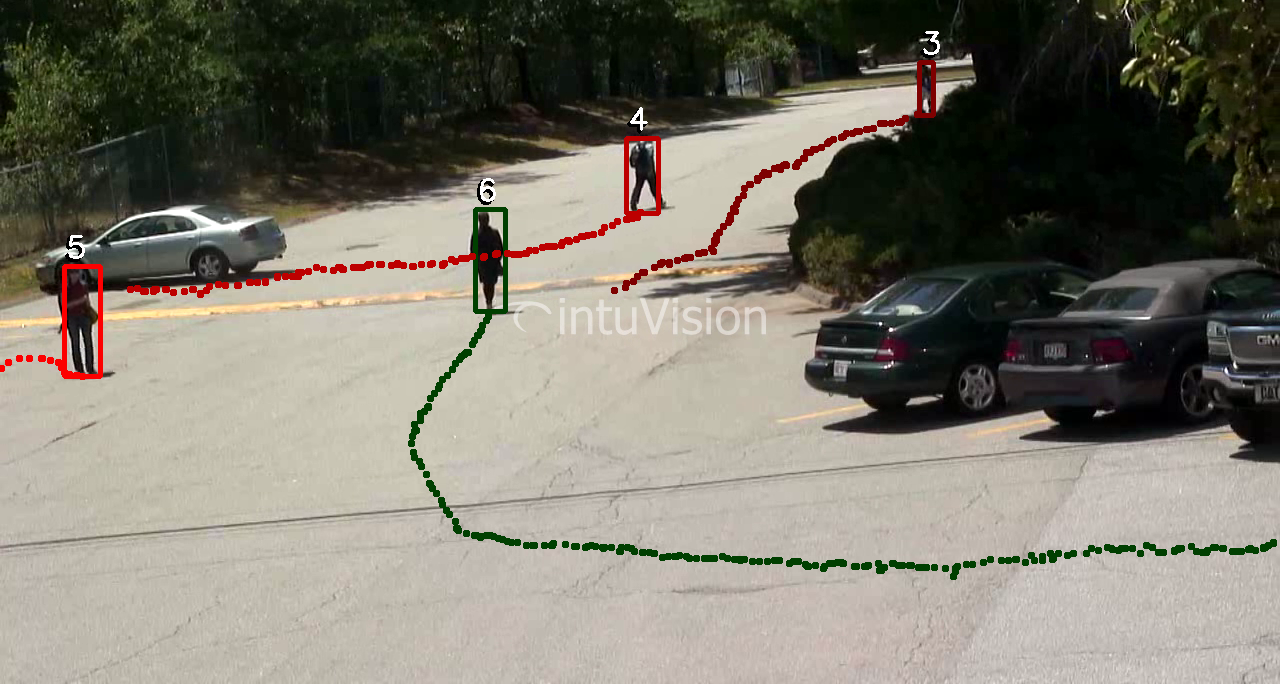
\includegraphics[width=6cm]{Figures/Tracking}
			};
		\end{tikzpicture}
	\end{columns}
	
	\vspace{0.3cm}
	
	\tiny
	
	\cite{Bloisi12} D. D. Bloisi \emph{et al.},  ``Independent Multimodal Background Subtraction'',
	CompIMAGE, 2012
\end{frame}

\begin{frame}
	\frametitle{PTracking}
	\framesubtitle{Pseudo-code}
	
	\begin{columns}[T]
		\column{.05\textwidth}
		
		\column{.55\textwidth}
		
		\only<1>
		{
			\begin{algorithm}[H]
				\tiny
				\KwIn{perceptions $ z_{s,t} $, local track numbers $ oi_{s,t-1} $, global track numbers $ OI_{s,t-1} $}
				\BlankLine
				\KwData{set of local particles $ \tilde{\xi}_{s,t} $, set of global particles $ \tilde{\xi}_{\mathcal{S'},t} $, sensor pose $ m_{s,t} $, local GMM set $ \mathcal{L} $, global GMM set $ \mathcal{G} $}
				\BlankLine
				\KwOut{global estimations $ x_{s,t} = (\boldsymbol{OI}_{s,t},\boldsymbol\Lambda_{s,t},\boldsymbol{M}_{s,t},\boldsymbol\Sigma_{s,t}) $}
				\BlankLine
				\Begin
				{
					\textcolor{darkgreen}{$ \tilde{\xi}_{s,t} \sim \pi_t (x_{s,t} | x_{s,t-1},z_{s,t},m_{s,t}) $}
					\BlankLine
					\textcolor{darkgreen}{Re-sample by using the SIR principle}\\
					\BlankLine
					\textcolor{darkgreen}{$ \mathcal{L} = KClusterize(\tilde{\xi}_{s,t}) $}
					\BlankLine
					\textcolor{darkgreen}{$ (\boldsymbol{oi}_{s,t},\boldsymbol\lambda_{s,t},\boldsymbol\mu_{s,t},\boldsymbol\sigma_{s,t}) = DataAssociation(\mathcal{L}, oi_{s,t-1}) $}
					\BlankLine
					\textcolor{darkgreen}{Communicate belief $ (\boldsymbol{oi}_{s,t},\boldsymbol\lambda_{s,t},\boldsymbol\mu_{s,t},\boldsymbol\sigma_{s,t}) $ to other agents}
				}
				\BlankLine
				\Begin
				{
					Collect $ \mathcal{L}_{S'} $ from a subset $ \mathcal{S'} \subseteq \mathcal{S} $ of
					sensors within a $ \Delta t $
					\BlankLine
					$ \tilde{\xi}_{\mathcal{S'},t} \sim \tilde\pi = \sum_{s \in \mathcal{S'}} \boldsymbol\lambda_{s,t} \, \mathcal{N} (\boldsymbol\mu_{s,t},\boldsymbol\sigma_{s,t}) $
					\BlankLine
					Re-sample by using the SIR principle\\
					\BlankLine
					$ \mathcal{G} = KClusterize(\tilde\xi_{{\mathcal{S'},t}}) $
					\BlankLine
					$ (\boldsymbol{OI}_{s,t},\boldsymbol\Lambda_{s,t},\boldsymbol{M}_{s,t},\boldsymbol\Sigma_{s,t}) = DataAssociation(\mathcal{G},OI_{s,t-1}) $
				}
			\end{algorithm}
			
			\column{.01\textwidth}
			
			\Huge
			\vspace{2.15cm}
			
			\begin{center}
				\textcolor{blue}{$ \Rightarrow $}
			\end{center}
			
			\column{.44\textwidth}
			
			\centering
			
			\begin{tikzpicture}
				\node at (0,0) [draw=black,ultra thick,inner sep=0pt]
				{
					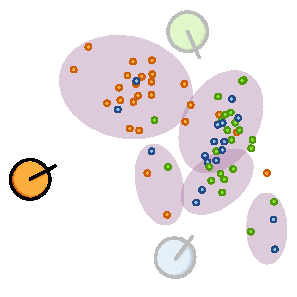
\includegraphics[width=3.3cm]{Figures/Mamot-1}
				};
				\node at (0,-3.5) [draw=black,ultra thick,inner sep=0pt]
				{
					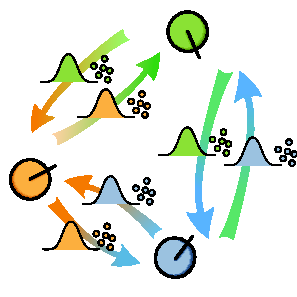
\includegraphics[width=3.3cm]{Figures/Mamot-2}
				};
			\end{tikzpicture}
		}
		
		\only<2->
		{
			\begin{algorithm}[H]
				\tiny
				\KwIn{perceptions $ z_{s,t} $, local track numbers $ oi_{s,t-1} $, global track numbers $ OI_{s,t-1} $}
				\BlankLine
				\KwData{set of local particles $ \tilde{\xi}_{s,t} $, set of global particles $ \tilde{\xi}_{\mathcal{S'},t} $, sensor pose $ m_{s,t} $, local GMM set $ \mathcal{L} $, global GMM set $ \mathcal{G} $}
				\BlankLine
				\KwOut{global estimations $ x_{s,t} = (\boldsymbol{OI}_{s,t},\boldsymbol\Lambda_{s,t},\boldsymbol{M}_{s,t},\boldsymbol\Sigma_{s,t}) $}
				\BlankLine
				\Begin
				{
					$ \tilde{\xi}_{s,t} \sim \pi_t (x_{s,t} | x_{s,t-1},z_{s,t},m_{s,t}) $
					\BlankLine
					Re-sample by using the SIR principle\\
					\BlankLine
					$ \mathcal{L} = KClusterize(\tilde{\xi}_{s,t}) $
					\BlankLine
					$ (\boldsymbol{oi}_{s,t},\boldsymbol\lambda_{s,t},\boldsymbol\mu_{s,t},\boldsymbol\sigma_{s,t}) = DataAssociation(\mathcal{L}, oi_{s,t-1}) $
					\BlankLine
					Communicate belief $ (\boldsymbol{oi}_{s,t},\boldsymbol\lambda_{s,t},\boldsymbol\mu_{s,t},\boldsymbol\sigma_{s,t}) $ to other agents
				}
				\BlankLine
				\Begin
				{
					\textcolor{lightred}{Collect $ \mathcal{L}_{S'} $ from a subset $ \mathcal{S'} \subseteq \mathcal{S} $ of sensors within a $ \Delta t $}
					\BlankLine
					\textcolor{lightred}{$ \tilde{\xi}_{\mathcal{S'},t} \sim \tilde\pi = \sum_{s \in \mathcal{S'}} \boldsymbol\lambda_{s,t} \, \mathcal{N} (\boldsymbol\mu_{s,t},\boldsymbol\sigma_{s,t}) $}
					\BlankLine
					\textcolor{lightred}{Re-sample by using the SIR principle}\\
					\BlankLine
					\textcolor{lightred}{$ \mathcal{G} = KClusterize(\tilde\xi_{{\mathcal{S'},t}}) $}
					\BlankLine
					\textcolor{lightred}{$ (\boldsymbol{OI}_{s,t},\boldsymbol\Lambda_{s,t},\boldsymbol{M}_{s,t},\boldsymbol\Sigma_{s,t}) = DataAssociation(\mathcal{G},OI_{s,t-1}) $}
				}
			\end{algorithm}
			
			\column{.01\textwidth}
			
			\Huge
			\vspace{2.15cm}
			
			\begin{center}
				\textcolor{blue}{$ \Rightarrow $}
			\end{center}
			
			\column{.44\textwidth}
			
			\centering
			
			\begin{tikzpicture}
				\node at (0,0) [draw=black,ultra thick,inner sep=0pt]
				{
					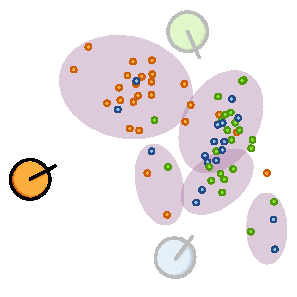
\includegraphics[width=3.3cm]{Figures/Mamot-1}
				};
				\node at (0,-3.5) [draw=black,ultra thick,inner sep=0pt]
				{
					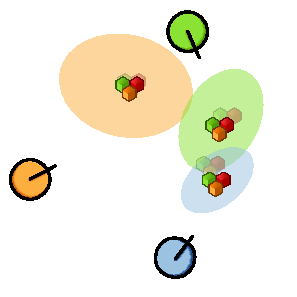
\includegraphics[width=3.3cm]{Figures/Mamot-3}
				};
			\end{tikzpicture}
		}
	\end{columns}
\end{frame}

\begin{frame}
	\frametitle{PTracking}
	\framesubtitle{Group Tracking}
	
	\begin{figure}
		\begin{tikzpicture}[map/.style={draw=black,ultra thick,inner sep=0pt}]
			\node at (0,0) [map] {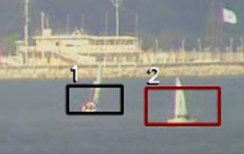
\includegraphics[width=0.32\linewidth]{Figures/GroupTracking-a}};
			\node at (4,0) [map] {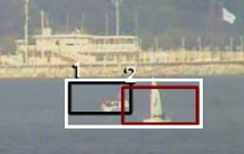
\includegraphics[width=0.32\linewidth]{Figures/GroupTracking-b}};
			\node at (8,0) [map] {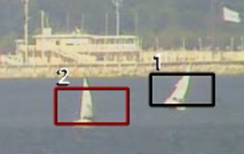
\includegraphics[width=0.32\linewidth]{Figures/GroupTracking-c}};
		\end{tikzpicture}
		\caption{Group tracking. Two sailing boats are going to cross each other. Occlusions are handled
				 considering the collapsing tracks to form a group, instead of tracking them
				 separately.}
	\end{figure}
\end{frame}

\begin{frame}
	\frametitle{KClusterize}
	\framesubtitle{Contributions}
	
	\Large
	
	\emph{KClusterize} has been designed aiming at fulfilling the following three requirements:
	
	\begin{enumerate}
		\item \textbf{Number} of objects to be detected \textbf{cannot} be known a priori
		\item \textbf{Low} computational load for real-time applications
		\item \textbf{Gaussian distribution} for each cluster
	\end{enumerate}
\end{frame}

\begin{frame}
	\frametitle{KClusterize}
	\framesubtitle{Typical Clustering Scenario}
	
	\vspace{0.5cm}
	
	\begin{figure}[!t]
		\begin{minipage}[l]{0.23\textwidth}
			\vspace*{\fill}
			\centering
			\subfigure[Analysed situation.]
			{
				\begin{tikzpicture}[map/.style={draw=white,ultra thick,inner sep=0pt}]
					\node at (0,0) [map]
					{
						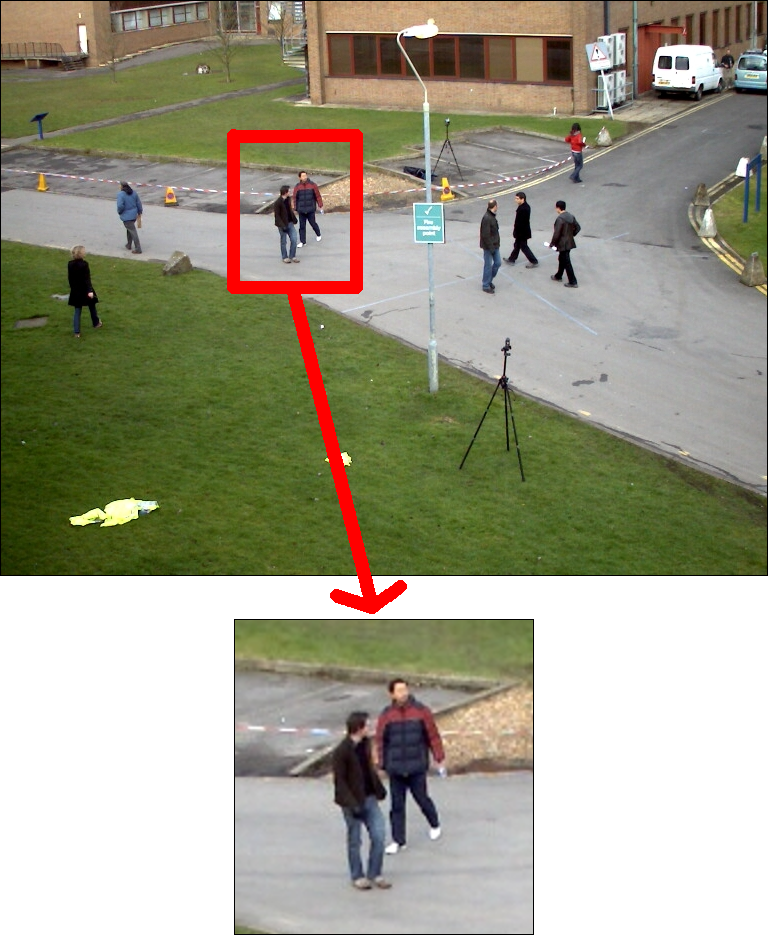
\includegraphics[width=\linewidth]{Figures/PETS-2009-Frame-0722-zoomed}
					};
				\end{tikzpicture}
			}
		\end{minipage}
		\hspace{0.1cm}
		\begin{minipage}[c]{0.74\textwidth}
			\subfigure[K-means with $ k = 2 $.]
			{
				\begin{tikzpicture}[map/.style={draw=white,ultra thick,inner sep=0pt}]
					\node at (0,0) [map]
					{
						\includegraphics[width=0.47\linewidth]{Figures/Kmeans-2.png}
					};
				\end{tikzpicture}
			}
			\hspace{-3.8mm}
			\subfigure[Hierarchical Clustering.]
			{
				\begin{tikzpicture}[map/.style={draw=white,ultra thick,inner sep=0pt}]
					\node at (0,0) [map]
					{
						\includegraphics[width=0.47\linewidth]{Figures/HierarchicalClustering.png}
					};
				\end{tikzpicture}
			}
			
			\subfigure[QT-Clustering.]
			{
				\begin{tikzpicture}[map/.style={draw=white,ultra thick,inner sep=0pt}]
					\node at (0,0) [map]
					{
						\includegraphics[width=0.47\linewidth]{Figures/QT-Clustering.png}
					};
				\end{tikzpicture}
			}
			\hspace{-3.8mm}
			\subfigure[KClusterize.]
			{
				\begin{tikzpicture}[map/.style={draw=white,ultra thick,inner sep=0pt}]
					\node at (0,0) [map]
					{
						\includegraphics[width=0.47\linewidth]{Figures/KClusterize.png}
					};
				\end{tikzpicture}
			}
		\end{minipage}
	\end{figure}
\end{frame}

\begin{frame}
	\frametitle{KClusterize}
	\framesubtitle{Clustering Speed}
	
	\begin{figure}[t]
		\begin{tikzpicture}[map/.style={draw=white,ultra thick,inner sep=0pt}]
			\node at (0,0) [map]
			{
				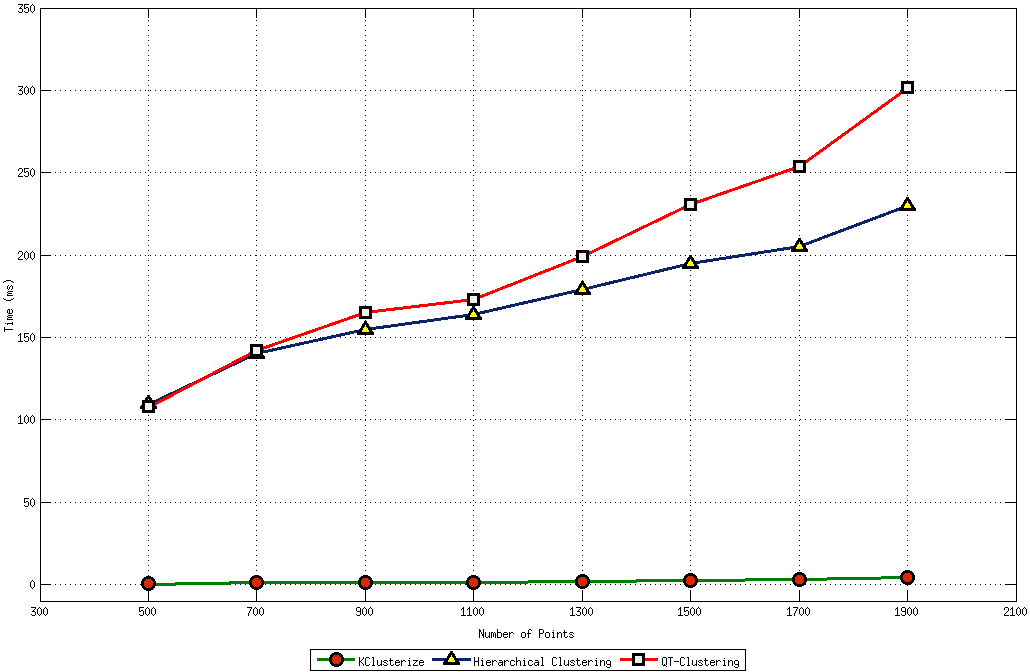
\includegraphics[width=0.88\linewidth]{Figures/ClusteringComparison}
			};
		\end{tikzpicture}
	\end{figure}
\end{frame}

\begin{frame}
	\frametitle{KClusterize}
	\framesubtitle{Cluster Gaussian Distribution}
	
	\vspace{0.3cm}
	
	\setcounter{subfigure}{0}
	
	\begin{figure}[!t]
		\centering
		\subfigure[Output of the algorithm on frame \#269.]
		{
			\begin{tikzpicture}[map/.style={draw=black,ultra thick,inner sep=0pt}]
				\node at (0,0) [map]
				{
					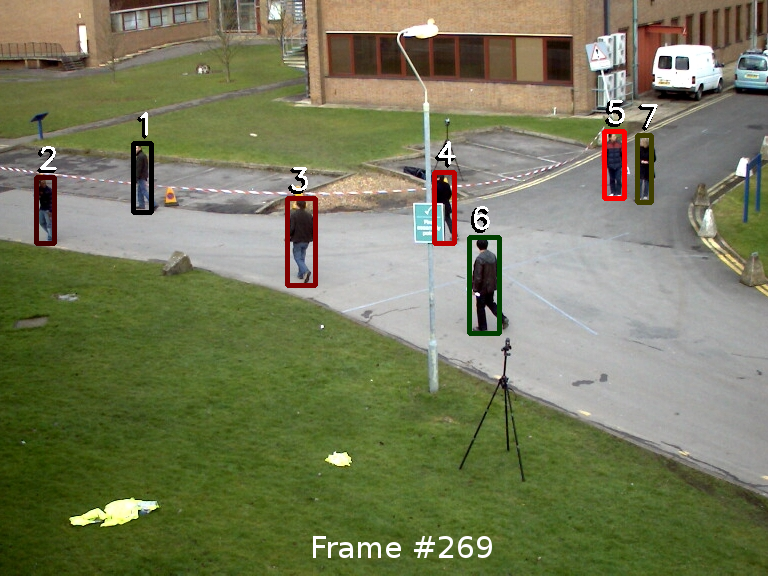
\includegraphics[width=0.48\linewidth]{Figures/KClusterize-Frame-0269-Output.png}
				};
			\end{tikzpicture}
		}
		\hspace{-3.8mm}
		\subfigure[A 2D visualization of frame \#269.]
		{
			\begin{tikzpicture}[map/.style={draw=white,ultra thick,inner sep=0pt}]
				\node at (0,0) [map]
				{
					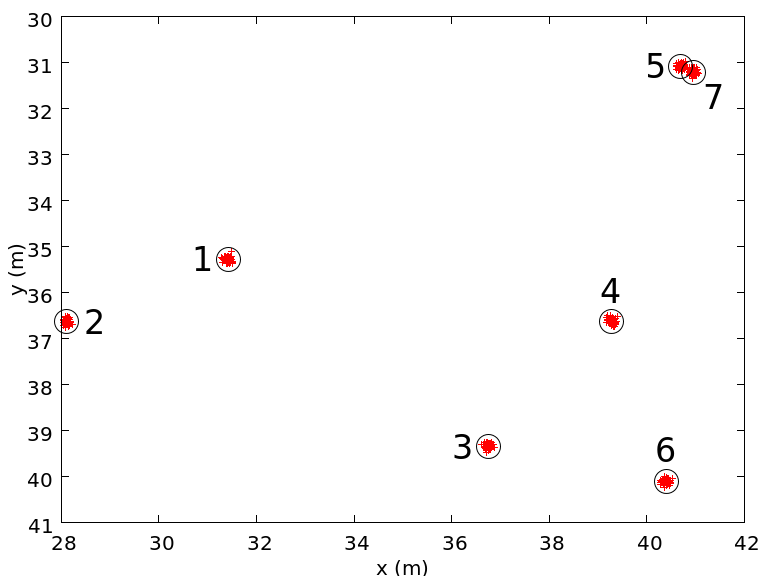
\includegraphics[width=0.48\linewidth]{Figures/KClusterize-Frame-0269-PlaneView.png}
				};
			\end{tikzpicture}
		}
	\end{figure}
\end{frame}

\section{Experimental Evaluation}

\begin{frame}
	\frametitle{Quantitative Evaluation}
	\framesubtitle{Scenarios}
	
	
\end{frame}

\section{Conclusions}

\begin{frame}
	\frametitle{Conclusions}
	
	\Large
	
	\vspace{0.3cm}
	
	We presented:
	
	\begin{enumerate}
		\item \emph{PTracking}, a novel \textbf{real-time} distributed tracker
		\item \textbf{Effective} framework for \textbf{predicting} future agent motions of
			  goal-oriented agents
	\end{enumerate}
	
	\vspace{0.2cm}
	
	\underline{\textbf{Main contributions}}
	
	\begin{itemize}
		\item Real-time, accurate and precise tracking
		\item Fully scalable design
		\item Prediction without prior annotation of scene semantics
		\item Non-uniform grids for state representation
		\item Efficient and scalable for on-robot implementation
	\end{itemize}
\end{frame}

\begin{frame}
	\frametitle{Future Work}
	
	\Large
	
	Possible future directions in terms of tracking could be:
	\begin{itemize}
		\item \textbf{Integration} of recent real-time \textbf{feature extractors} in the data
			  association module
		\item \textbf{Generation} of a \textbf{3D model} by merging information coming from multiple
			  sources
	\end{itemize}
	
	while, in terms of prediction of future agent motions could be the employment of \textbf{more
	sophisticated} \emph{IRL} alternatives within the overall proposed framework.\\
\end{frame}

\logo{}

\begin{frame}
	\frametitle{Major Reviewers' Comments}
	
	\large
	
	\textbf{Rev.}\\
	``For some experiments, comparisons are only made with various versions of the same algorithms.''
	
	\vspace{0.3cm}
	
	\textbf{Rev.}\\
	``The benefits of the method are shown for activity forecasting applications, intention prediction,
	and for constructing interactive costmaps to guide robot navigation. The latter applications
	represent significant contributions in robotics. Some additional discussion of the assumptions being  
	employed would be useful. Specifically, the joint optimization seems to assume more coordination
	than, e.g., humans have when they navigate (often sub-­optimally).'' \\
\end{frame}

\logo
{
	\begin{tikzpicture}
		\hspace{0.09cm}
		\node at (-1,0) [draw=white,ultra thick,inner sep=0pt]
		{
			
\includegraphics[height=1cm]{ThemeFigs/Sapienza}
		};
		\node at (0,0) [draw=white,ultra thick,inner sep=0pt]
		{
			
\includegraphics[height=1cm]{ThemeFigs/Edinburgh}
		};
	\end{tikzpicture}
	\vspace{199.1pt}
}

\begin{frame}
	\frametitle{Full List of Publications}
	
	\vspace{-0.2cm}
	
	\begin{columns}[t]
		\column{0.48\textwidth}
		
		\tiny
		
		\textcolor{red}{\textbf{\underline{Journal}}}
		
		\vspace{0.1cm}
		
		\textbf{1. Multi-Robot Surveillance through a Distributed Sensor Network}, A. Pennisi, F.
		Previtali, C. Gennari, D. D. Bloisi, L. Iocchi, F. Ficarola, A. Vitaletti, D. Nardi \\
		\emph{Journal of Studies in Computational Intelligence, 2015}
		
		\vspace{0.15cm}
		
		\textbf{2. Distributed Sensor Network for Multi-Robot Surveillance}, A. Pennisi, F. Previtali,
		F. Ficarola, D. D. Bloisi, L. Iocchi, A. Vitaletti \\
		\emph{Procedia Computer Science, 2014}
		
		\vspace{0.2cm}
		
		\textcolor{red}{\textbf{\underline{Conference}}}
		
		\vspace{0.1cm}
		
		\textbf{3. PTracking: Distributed Multi-Agent Multi-Object Tracking through Multi-Clustered
		Particle Filtering}, F. Previtali, L. Iocchi \\
		\emph{IEEE Conference on Multisensor Fusion and Integration, 2015}
		
		\vspace{0.15cm}
		
		\textbf{4. Disambiguating Localization Symmetry through a Multi-Clustered Particle Filtering},
		F. Previtali, G. Gemignani, L. Iocchi, D. Nardi \\
		\emph{IEEE Conference on Multisensor Fusion and Integration, 2015}
		
		\vspace{0.15cm}
		
		\textbf{5. Counterfactual Reasoning about Intent for Interactive Navigation in Dynamic
		Environments}, A. Bordallo, F. Previtali, N. Nardelli, S. Ramamoorthy \\
		\emph{IEEE Conference on Intelligent Robots and Systems, 2015}
		
		\vspace{0.15cm}
		
		\textbf{6. IRL-based Prediction of Goals for Dynamic Environments}, F. Previtali, A. Bordallo,
		S. Ramamoorthy \\
		\emph{Machine Learning for Social Robotics at ICRA, 2015}
		
		\column{0.53\textwidth}
		
		\vspace{0.34cm}
		
		\tiny
		
		\textbf{7. Real-Time Adaptive Background Modeling in Fast Changing Conditions}, A. Pennisi, F.
		Previtali, D. D. Bloisi, L. Iocchi \\
		\emph{Conference on Advanced Video and Signal based Surveillance, 2015}
		
		\vspace{0.2cm}
		
		\textcolor{red}{\textbf{\underline{Submitted}}}
		
		\vspace{0.1cm}
		
		\textbf{8. A Distributed Approach for Real-Time Multi-Camera Multi-Object Tracking}, F.
		Previtali, D. D. Bloisi, L. Iocchi \\
		\emph{Journal on Machine Vision and Applications}
		
		\vspace{0.15cm}
		
		\textbf{9. Enhancing Automatic Maritime Surveillance Systems with Visual Information}, D. D.
		Bloisi, F. Previtali, A. Pennisi, D. Nardi, M. Fiorini \\
		\emph{Transaction on Intelligent Transportation Systems}
		
		\vspace{0.15cm}
		
		\textbf{10. Predicting Future Agent Motions for Dynamic Environments}, F. Previtali, A.
		Bordallo, L. Iocchi, S. Ramamoorthy \\
		\emph{IEEE Conference on Intelligent Robots and Systems}
		
		\vspace{0.15cm}
		
		\textbf{11. Interactive Costmaps: Integrating Prediction and Planning with Counterfactual
		Reasoning}, A. Bordallo, F. Previtali, S. Ramamoorthy \\
		\emph{IEEE Conference on Intelligent Robots and Systems}
	\end{columns}
\end{frame}

\logo{}

\begin{frame}
	\frametitle{That's all!}
	
	\begin{figure}
		\centering
		\begin{tikzpicture}
			\node at (0,0) [draw=white,ultra thick,inner sep=0pt]
			{
				
\includegraphics[width=0.8\linewidth]{Figures/Question}
			};
		\end{tikzpicture}
	\end{figure}
\end{frame}


\end{document}
